

The \textbf{monitoring module} is responsible for storing metrics, resolving queries regarding stored metrics, removing expired metrics, periodically evaluating registered alarms, triggering callbacks which the API then propagates to the client, among other features which we will discuss now in more detail.

We believe it is, however, important to remember that the focus of this work is to provide a usable proof-of-concept of a decentralized monitoring framework, targeted for decentralized resource management solutions. Consequently, the focus of this module is to provide just enough functionality for a proof of concept, namely in aspects such as the storage of metrics in disk or the efficiency of the query language, which are interesting research challenges by themselves, however, are orthogonal to the work presented here. 

This module is composed by three different components (illustrated in Figure~\ref{fig:mon_module_overview}): the \textbf{query engine}, the \textbf{time-series database} (TSDB), and the \textbf{alert manager}, whose roles in the system we now briefly explain:

\begin{figure}[htbp]
    \centering
    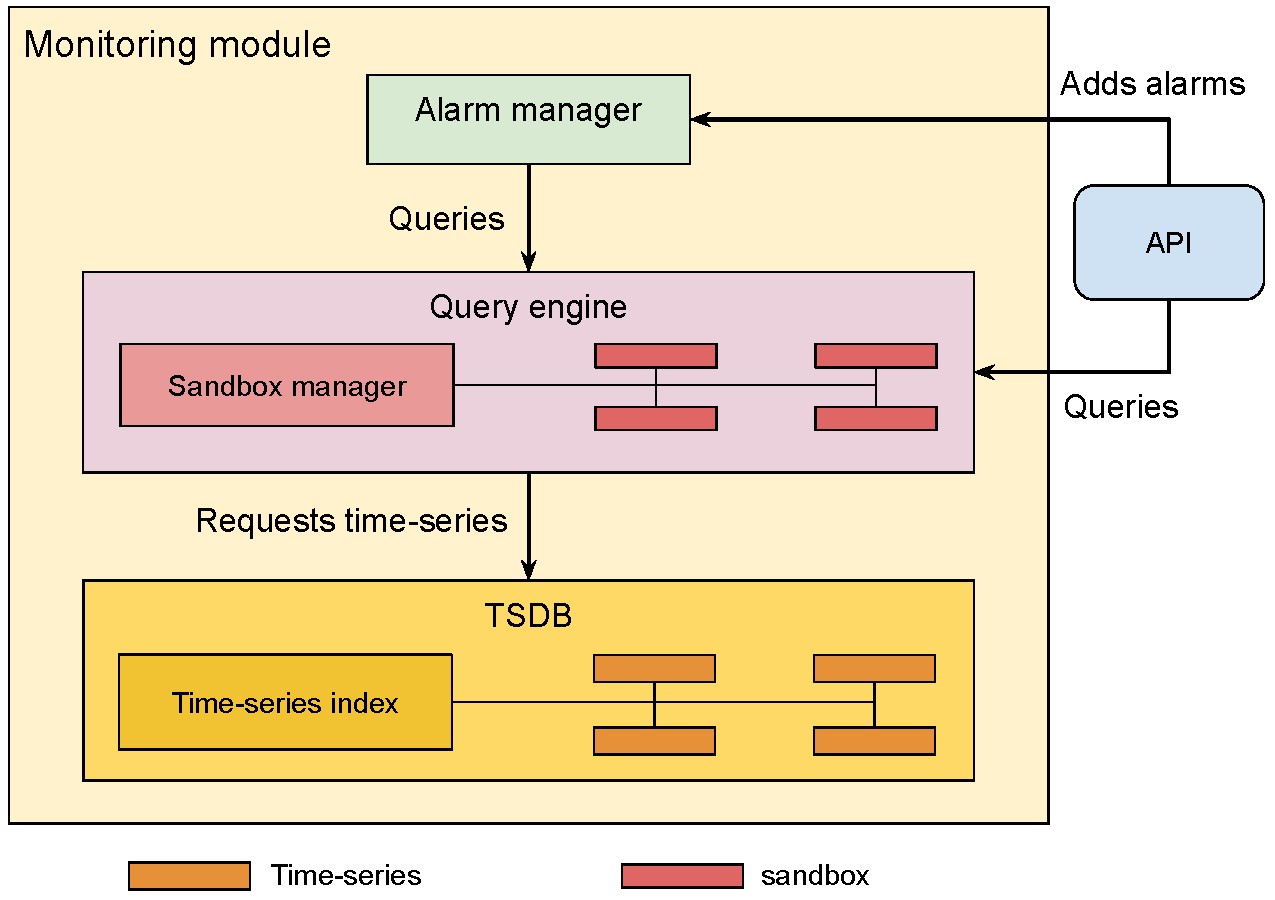
\includegraphics[width=\textwidth]{Chapters/mon_module/images/Monitoring_module.pdf}
    \caption{An overview of the monitoring module}
    \label{fig:mon_module_overview}
\end{figure}

\begin{enumerate}
    
    \item The \textbf{time-series database} allows the insertion and retrieval of time-series data from the framework. This time-series database employs an in-memory index to retrieve one or more time-series according to a set of parameters. This component is responsible for storing and managing the information (e.g., expiring outdated entries) supplied by the applications and the decentralized aggregation protocol.

    \item The \textbf{query engine} is the component tasked with resolving queries made to the time-series database. This component maintains a set of sandboxes that evaluate user-provisioned queries that both extract data from the database and apply aggregation functions to it.
    
    \item Finally, the \textbf{alert manager} manages the alarms registered through the API. In sum, this component periodically verifies the issued alarms' query using the \textbf{query engine} and propagates an event to the client whenever the condition is verified.
     
\end{enumerate}

In order to ease the explanation of these components, we first detail the structure of the metrics used in this framework, which has a similar structure to the metric types provided by InfluxDB~\cite{influxdb_data_elements}. 

\subsection{Metric  structure}

In DeMMon, a metric is composed of four elements: first, the \textbf{name}, which is a string denoting the name of the stored information, the name should be a human-readable name which is self-describing (e.g. ``CPU-USAGE''). The second element are the metric \textbf{tags}, which are a set of string pairs denoting attributes related to the metric that is stored, (e.g. the hostname or cluster name of the node that emitted it), next, we have the \textbf{value}, which contains the data associated with the observed metric, and finally, we have the  \textbf{timestamp}, that contains the time at which the observation was taken. A typical example of a metric in the devised framework would be: name: ``CPU-Usage''; tags: <host:nodeX>, value: 0.3, timestamp: ``1609960731''.

We believe it is important to mention that in order to remain as flexible as possible, the metric values do not have a defined type. In this system, clients may use custom types (as long as they are serializable using the JSON package provided by the Golang~\cite{golang} package). This allows the devised framework to represent a multitude of different information types, such as histograms, strings, string maps, among others, which offers a higher degree of flexibility for using this framework. For example, a decentralized service management system aimed at deploying service replicas in close proximity to the clients may use, for example, a histogram with pre-determined geographical classes. This way, this system would have a data structure that would ease finding a node in the desired geographical area.

Provided with the metric structure, we now explain how these are stored in the system. 

\subsection{Time-series database}  \label{sec:mon_module:tsdb}

In DeMMon, time-series are sequences taken at successive equally spaced points in time. In this system, time-series are stored only in memory and are indexed as a function of their name and tags.

In order for a certain metric (composed by: name, tags, and periodicity) to be inserted into the database, a \textbf{bucket} must first be created. A bucket is essentially a component that holds all time-series data with a certain name, periodicity and capacity. The periodicity denotes the interval at which the sequences of points are spaced (in time) and the capacity denotes the number of points stored in each sequence. For example, a time-series with a 5-second periodicity and a capacity of 12 holds all points from the last minute. Limiting the number of points per series allows the system to pre-allocate the memory necessary (using an array) for each time-series at the time of its creation.

Within a bucket, metrics are stored in a map and indexed by their tags. This is done by generating keys that are equal for each similar tag set, independent of its order: whenever a metric is inserted, the tag pairs are sorted alphabetically (by their key) and concatenated into a single string, producing the resulting metric key. Then, using the metric key, the metric value is inserted into the corresponding time-series (a new time-series is created for that tag set if there was none previously in the system).

Time-series advance time in an on-demand manner, meaning that, before returning values for any read or write request from a time-series, the system first verifies if its' oldest value has a timestamp outside of the time-series window (as time has passed since the last check). If it has, the system iterates the time-series' points from its oldest to the newest point and removes all points outside its time window. In order to remove unused time-series from the system, and decrease DeMMons' memory footprint, the time-series database component also periodically advances the time-series in time and removes any time-series that has become empty.

Concurrency is handled by using locking mechanisms, where operations that do not affect the state of the time-series are executed concurrently, and operations that would otherwise change the time-series status are executed sequentially. 

\subsection{Query engine} \label{sec:mon_module:query_engine}

The query engine is a sub-component of the monitoring module, and it is responsible for evaluating the supplied text-based queries, transforming them into sets of instructions, and determining the final query result by executing the instructions. Keeping in mind the fact that the focus of this work is not the performance of the metric storage or the query language and that it is still a focal point of this work to be as flexible as possible in the query language, we opted for using javascript-based sandboxes to perform this work. This means that user-provided queries are essentially javascript code, and consequently, users have infinite control over the behaviour of their queries, provided these do not exceed the query timeout.

To provide this functionality, we opted for using the package Otto~\cite{otto}. This package provides access to javascript ``virtual machines'' that essentially parse a string containing javascript code, and produce an AST from the parsed code. The produced ASTs are then executed and their result is returned by the VM. In order to allow users to access the time-series stored in the TSDB, the query engine provides every Otto virtual machine access to the following functions, which return time-series from the database:

\begin{enumerate}

    \item Select(Bucket\_Name, <Tag\_set\_regex), this function returns the time-series that are in the supplied bucket matching the provided tag set regex. The way the tag set regex matching works is: for every time series present in the specified bucket, if all of the tag keys in the supplied regex match all of the time series tags, then the time series is returned. An example of the usage of this function would be, for example: ``select(CPU\_USAGE, <host:.*, cluster:cluster1>)''

    \item SelectLast(Bucket\_Name, <Tag\_set\_regex>), this function behaves similarly to Select, however, it only returns the last inserted point in all matched time series.
    
    \item SelectRange(Bucket\_Name, <Tag\_set\_regex>, startDate, endDate), this function behaves similarly to ``Select'' and ``SelectLast'', however, it allows users to only extract a certain time-window from the matching time-series. To do so, it takes an additional argument, consisting of a time range, used to filter the points to return to the client.
    
\end{enumerate}

% With these three functions, clients can select either partial sets of points or the totality of points from every time series stored in the database, which are then usable in the javascript code.  

We believe these functions cover the most common use cases for metric selection. These metrics, upon selection, can then be aggregated in any way the user specifies in the query (since they are composed of user-defined code). In order to ease the design of queries and prevent developers from rewriting the same aggregation functions, the query engine also provides some aggregation primitives which can be applied to one or more time-series such as: Max, Min, and Average.

After the selection asnd aggregation of metrics, the resulting values are returned by placing them in a variable denoted ``result'' (in the user-defined code). Any query executed in DeMMon can only result in one of two types: a single time series or an array of time series (following an interface defined by DeMMon). Given this, in order to allow the creation of new time series that follow this interface during the query process, there are two additional functions supplied to the virtual machines: the first is called ``NewTimeSeries'', which creates a new time series, this function takes as arguments the name, tags and values which will integrate the time series; second, we have the function called ``NewObservable'' which takes a value of any type and a timestamp, and creates a new metric point which can be added to time series.

 With this, we now provide some examples of possible queries along with a brief description of what they do:

\begin{enumerate}
    \item ``Avg(SelectLast(CPU\_USAGE, <host:.*, cluster:cluster1>))'' this query selects the metrics with the name ``CPU\_USAGE'' for all hosts which belong to cluster with name ``cluster1'' and returns the average of all the points.
    
    \item ``SelectLast(Nr\_services, <tenant:tenant10>, startDate, endDate)'' this query returns the timeseries for the metric called ``Nr\_services'' for the tenant with name ``tentant10'' during the provided time range.

    \item ``SelectLast(Nr\_replicas, <tenant:tenant10,service:service10>)'' this query returns the timeseries for the metric called ``Nr\_replicas'' for the tenant with name ``tentant10'' and service named ``service10'' during the provided time range.
    
\end{enumerate}

With this, clients are able to obtain and manipulate data from the time series database using text-based queries. Furthermore, as the type of the value of each metric is not enforced, clients may store their metrics in custom data structures, tailored for their specific use-cases.

\subsection{Alarm manager} \label{sec:mon_module:alarm_monitor}

The alert manager is the last component of the monitoring module, it is responsible for managing the \textbf{alarms} issued to the monitoring module. Alarms are essentially sets of parameters that contain, among other parameters, a condition to observe (e.g. the percentage of CPU usage) and a periodicity to observe this condition. Alarms are paramount to prevent applications from having to periodically query DeMMon to verify the condition themselves, effectively saving bandwidth. This component is essentially responsible for periodically verifying these alarms and issuing notifications to the client whenever their conditions are verified. 

In DeMMon, an alarm contains the following parameters: 

\begin{enumerate}
    \item \textbf{Condition}. This is essentially a query (explained in Section~\ref{sec:mon_module:query_engine}) that must return a boolean value.
    
    \item \textbf{Periodicity}. The periodicity denotes how often the condition is evaluated and how often notifications are sent to the client that issued the alarm
    
    \item \textbf{Backoff time}. The backoff time is a time duration that bounds the rate at which the monitoring module emits notifications, which would otherwise happen at the alarm periodicity every time the alarm is verified (e.g. if the supplied periodicity is low).
    
    \item \textbf{Watch list}. The watch list is a set that, for every item, contains both a name and a set of tag filters. Whenever the alarm manager receives an alarm containing a watch list, in addition to performing the verification at the specified periodicity, it also performs the verification whenever any time series matching the watch list is changed. The rates at which the alarm is verified in this manner also respects the backoff time.
    
    \item \textbf{CheckPeriodic}. CheckPeriodic is a boolean variable denoting if the alarm should be verified periodically. When false, the alarm manager does not check the metrics at every \textbf{``periodicity''} seconds (defined previously), effectively saving CPU time. This option is meant to be used together with the watch list, for example, for checking a parameter that is rarely altered.
    
\end{enumerate}

The monitoring module, whenever it receives the registration of a new alarm, essentially adds it to a priority queue containing all the alarms. This priority queue uses the time of reception of the alarms plus their periodicity as their key to the queue. With this, alarms are sorted by the time at which they need to be verified. The monitoring module continuously obtains and removes the first item of the queue, containing the next alarm to verify out of all issued alarms and waits until it is time of verification of that alarm (i.e. the time of reception of the alarm plus its periodicity). Ater this, it evaluates the condition (emitting a notification to the client if the condition is verified), and re-adds the alarm to the queue with a key corresponding to the current time plus the alarms' periodicity. Whenever an alarm is verified, and the result of its condition returns ``true'', the alarm manager first verifies if it has emitted a notification for that alarm in the last ``Backoff time'' duration, and issues a notification to the client if it has not.